% Root file used ashow macros
\documentclass{beamer}
\usepackage{tikz}
\usetikzlibrary{calc,arrows.meta,patterns}
\usepackage{xcolor}
\usepackage{multicol}
\usepackage{amsmath}

% ================================================================
% Answer-overlay helpers
% ================================================================
\newcommand{\ablank}[1]{%
  \alt<2>{\textcolor{red}{#1}}{\underline{\phantom{#1}}}%
}
\newcommand{\ashow}[1]{\uncover<2->{\textcolor{red}{\small #1}}}
\newcommand{\ashowq}[1]{\alt<2->{\textcolor{red}{\small #1}}{?}}

% Answers drawn straight on to a TikZ diagram, revealed on overlay 2 like \ashow.
% Space is reserved on overlay 1, so the diagram does not move between slides.
\usetikzlibrary{overlay-beamer-styles}
\tikzset{
  ans/.style     = {red, thick, visible on=<2->},
  ansfill/.style = {red!15, visible on=<2->},
  anslab/.style  = {red, font=\tiny, visible on=<2->},
}

\title{Circles: Area, Squaring \& Pi}
\author{}
\date{}

\begin{document}

\frame{\titlepage}

%------------------------------------------------
% CONTENTS
%------------------------------------------------
\begin{frame}{Contents}
\small
\begin{columns}[T]
\column{0.5\textwidth}
\textbf{Questions and short answers}
\begin{itemize}
  \item \hyperlink{q-st1}{\beamergotobutton{Starter 1}}
  \item \hyperlink{q-st2}{\beamergotobutton{Starter 2}}
  \item \hyperlink{q-st3}{\beamergotobutton{Starter 3}}
  \item \hyperlink{q-st4}{\beamergotobutton{Starter 4}}
\end{itemize}

\column{0.5\textwidth}
\textbf{Worked solutions}
\begin{itemize}
  \item \hyperlink{work-st1}{\beamergotobutton{Starter 1}}
  \item \hyperlink{work-st2}{\beamergotobutton{Starter 2}}
  \item \hyperlink{work-st3}{\beamergotobutton{Starter 3}}
  \item \hyperlink{work-st4}{\beamergotobutton{Starter 4}}
\end{itemize}
\end{columns}
\end{frame}

%------------------------------------------------
% STARTER 1
%------------------------------------------------
\begin{frame}{Starter 1}
\hypertarget{q-st1}{}

\vspace{-2em}

\begin{columns}

\column{0.35\textwidth}
\begin{center}
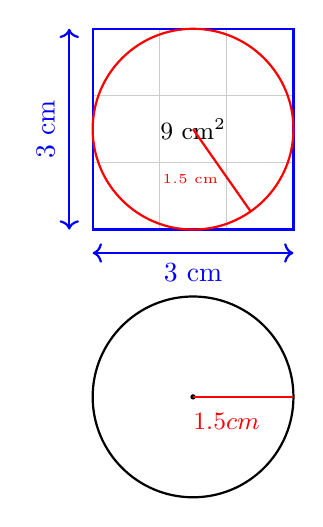
\begin{tikzpicture}[scale=0.85]
  % Grid of squares to illustrate squaring / area idea
  \draw[gray!40, thin] (0,0) grid (3,3);
  \draw[thick, blue] (0,0) rectangle (3,3);
  \draw[blue, thick, <->] (0,-0.35) -- (3,-0.35);
  \node[blue] at (1.5,-0.65) {$3$ cm};
  \draw[blue, thick, <->] (-0.35,0) -- (-0.35,3);
  \node[blue, rotate=90] at (-0.7,1.5) {$3$ cm};
  \node at (1.5,1.5) {\small $9$ cm$^2$};

  % Small circle below for context
  \draw[thick] (1.5,-2.5) circle (1.5cm);
  \fill (1.5,-2.5) circle (0.04);
  \draw[red, thick] (1.5,-2.5) -- ++(0:1.5);
  \node[red, below] at (2,-2.6) {\small $1.5cm$};

% --- Q9 answer: the r = 1.5 cm circle drawn inside the 3 cm square ---
\draw[ans] (1.5,1.5) circle (1.5cm);
\draw[ans] (1.5,1.5) -- ++(-55:1.5);
\node[anslab, left] at (2.02,0.76) {$1.5$ cm};
\end{tikzpicture}
\end{center}

\column{0.65\textwidth}
\small
\begin{enumerate}
  \begin{multicols}{2}
    \item $4 \times 4 = \ashowq{16}$
    \item $7 \times 7 = \ashowq{49}$
  \end{multicols}
  \begin{multicols}{2}
    \item $10^2 = \ashowq{100}$
    \item $3^2 = \ashowq{9}$
  \end{multicols}
  \item $2 \times 6$ and $6^2$ --- are these the same? \ashow{No: $12\neq 36$.}
  \begin{multicols}{2}
  \item $3.14 \times 9=\ablank{28.26}$
  \item $3.14 \times 25=\ablank{78.5}$
  \end{multicols}
\end{enumerate}
\vspace{-1em}
\begin{enumerate}
  \setcounter{enumi}{6}
  \item A circle has \textbf{diameter} $14$ cm. Find: \newline{} (a) the radius \ablank{7\,\text{cm}} \newline{} (b) the circumference \ablank{43.96\,\text{cm}}. ($\pi \approx 3.14$)
  \item A circle has \textbf{radius} $5$ cm. What is the circumference? \ablank{31.4\,\text{cm}}
  \item The square has side $3$ cm and area $9$ cm$^2$. A circle has radius $1.5$ cm. Is the circle's area more or less than $9$ cm$^2$? \ashow{Less: $\pi(1.5)^2 \approx 7.07$ cm$^2$.}
\end{enumerate}

\end{columns}
\end{frame}

\begin{frame}{Worked Solution: Starter 1, Question 1}
\hypertarget{work-st1}{}
\textbf{Question:} \(4 \times 4 = \ashowq{16}\)

\textbf{Worked Solution:} \ashow{\(4 \times 4 = 16\) because \(4+4+4+4=16\).}
\end{frame}

\begin{frame}{Worked Solution: Starter 1, Question 2}
\textbf{Question:} \(7 \times 7 = \ashowq{49}\)

\textbf{Worked Solution:} \ashow{\(7 \times 7 = 49\), from the \(7\) times table or \(7+7+7+7+7+7+7=49\).}
\end{frame}

\begin{frame}{Worked Solution: Starter 1, Question 3}
\textbf{Question:} \(10^2 = \ashowq{100}\)

\textbf{Worked Solution:} \ashow{\(10^2 = 10 \times 10 = 100\).}
\end{frame}

\begin{frame}{Worked Solution: Starter 1, Question 4}
\textbf{Question:} \(3^2 = \ashowq{9}\)

\textbf{Worked Solution:} \ashow{\(3^2 = 3 \times 3 = 9\).}
\end{frame}

\begin{frame}{Worked Solution: Starter 1, Question 5}
\textbf{Question:} Are \(2 \times 6\) and \(6^2\) the same?

\textbf{Worked Solution:} \ashow{No. \(2\times 6 = 12\), while \(6^2 = 36\). Since \(12 \neq 36\), they are not the same.}
\end{frame}

\begin{frame}{Worked Solution: Starter 1, Question 6}
\textbf{Question:} \(3.14 \times 9 = \ablank{28.26}\)

\textbf{Worked Solution:} \ashow{\(3.14 \times 9 = 3.14 \times (10-1) = 31.4 - 3.14 = 28.26\).}
\end{frame}

\begin{frame}{Worked Solution: Starter 1, Question 7}
\textbf{Question:} \(3.14 \times 25 = \ablank{78.5}\)

\textbf{Worked Solution:} \ashow{\(3.14 \times 25 = 3.14 \times \frac{100}{4} = \frac{314}{4} = 78.5\).}
\end{frame}

\begin{frame}{Worked Solution: Starter 1, Question 8}
\textbf{Question:} A circle has diameter \(14\) cm. Find: (a) the radius \ablank{\(7\,\text{cm}\)} and (b) the circumference \ablank{\(43.96\,\text{cm}\)}. (\(\pi \approx 3.14\))

\textbf{Worked Solution:} \ashow{Radius \(= \frac{14}{2} = 7\) cm. Circumference \(= \pi d = 3.14 \times 14 = 43.96\) cm.}
\end{frame}

\begin{frame}{Worked Solution: Starter 1, Question 9}
\textbf{Question:} A circle has radius \(5\) cm. What is the circumference? \ablank{\(31.4\,\text{cm}\)}

\textbf{Worked Solution:} \ashow{\(C = 2\pi r = 2 \times 3.14 \times 5 = 31.4\) cm.}
\end{frame}

%------------------------------------------------
% STARTER 2
%------------------------------------------------
\begin{frame}{Starter 2}
\hypertarget{q-st2}{}

\begin{columns}

\column{0.35\textwidth}
\begin{center}
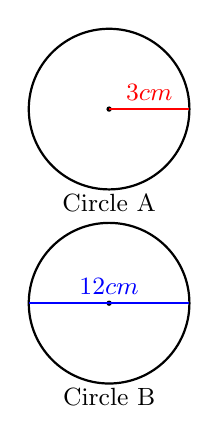
\begin{tikzpicture}[scale=0.85]

  % Circle A — radius labelled
  \draw[thick] (0,2.5) circle (1.2cm);
  \fill (0,2.5) circle (0.04);
  \draw[red, thick] (0,2.5) -- ++(0:1.2);
  \node[red] at (0.6, 2.75) {\small $3cm$};
  \node at (0, 1.1) {\small Circle A};

  % Circle B — diameter labelled
  \draw[thick] (0,-0.4) circle (1.2cm);
  \fill (0,-0.4) circle (0.04);
  \draw[blue, thick] (-1.2,-0.4) -- (1.2,-0.4);
  \node[blue] at (0,-0.15) {\small $12cm$};
  \node at (0,-1.8) {\small Circle B};

\end{tikzpicture}
\end{center}

\column{0.65\textwidth}
\small
\begin{enumerate}
  \begin{multicols}{2}
    \item Halve $12$ cm \ablank{6\,\text{cm}}
    \item Halve $9.4$ cm \ablank{4.7\,\text{cm}}
  \end{multicols}
  \begin{multicols}{2}
    \item $6^2 = \ashowq{36}$
    \item $1.5^2 = \ashowq{2.25}$
  \item $3 \times 4^2=\ablank{48}$
  \item True or false? $\pi \times (2r) = 2 \times \pi \times r$ \ashow{True}
  \end{multicols}
\end{enumerate}
\vspace{-2em}
\begin{enumerate}
  \setcounter{enumi}{6}
  \item Consider circle A \newline{} (a) What is the circumference? \ablank{18.84\,\text{cm}} \newline{} (b) What is the area? \ablank{$28.26\,\text{cm}^2$}
  \item Consider circle B \newline{} (a) What is the circumference? \ablank{37.68\,\text{cm}} \newline{} (b) What is the area? \ablank{$113.04\,\text{cm}^2$}
  \item Is the ratio of the cirumferences of circle's A and B the same as the ratio of the areas? \ashow{No: $1:2$ vs $1:4$.}
\end{enumerate}

\end{columns}
\end{frame}

\begin{frame}{Worked Solution: Starter 2, Question 1}
\hypertarget{work-st2}{}
\textbf{Question:} Halve \(12\) cm. \ablank{\(6\,\text{cm}\)}

\textbf{Worked Solution:} \ashow{\(12 \div 2 = 6\), so the answer is \(6\) cm.}
\end{frame}

\begin{frame}{Worked Solution: Starter 2, Question 2}
\textbf{Question:} Halve \(9.4\) cm. \ablank{\(4.7\,\text{cm}\)}

\textbf{Worked Solution:} \ashow{\(9.4 \div 2 = 4.7\), so the answer is \(4.7\) cm.}
\end{frame}

\begin{frame}{Worked Solution: Starter 2, Question 3}
\textbf{Question:} \(6^2 = \ashowq{36}\)

\textbf{Worked Solution:} \ashow{\(6^2 = 6 \times 6 = 36\).}
\end{frame}

\begin{frame}{Worked Solution: Starter 2, Question 4}
\textbf{Question:} \(1.5^2 = \ashowq{2.25}\)

\textbf{Worked Solution:} \ashow{\(1.5 \times 1.5 = 2.25\).}
\end{frame}

\begin{frame}{Worked Solution: Starter 2, Question 5}
\textbf{Question:} \(3 \times 4^2 = \ablank{48}\)

\textbf{Worked Solution:} \ashow{Square first: \(4^2 = 16\), then \(3 \times 16 = 48\).}
\end{frame}

\begin{frame}{Worked Solution: Starter 2, Question 6}
\textbf{Question:} True or false? \(\pi \times (2r) = 2 \times \pi \times r\)

\textbf{Worked Solution:} \ashow{True. By commutativity, \(\pi(2r) = 2\pi r\), so both sides are equal.}
\end{frame}

\begin{frame}{Worked Solution: Starter 2, Question 7}
\textbf{Question:} Circle A has radius \(3\) cm. Find: (a) the circumference \ablank{\(18.84\,\text{cm}\)} and (b) the area \ablank{\(28.26\,\text{cm}^2\)}.

\textbf{Worked Solution:} \ashow{\(C = 2\pi r = 2 \times 3.14 \times 3 = 18.84\) cm. \(A = \pi r^2 = 3.14 \times 3^2 = 3.14 \times 9 = 28.26\) cm\(^2\).}
\end{frame}

\begin{frame}{Worked Solution: Starter 2, Question 8}
\textbf{Question:} Circle B has diameter \(12\) cm. Find: (a) the circumference \ablank{\(37.68\,\text{cm}\)} and (b) the area \ablank{\(113.04\,\text{cm}^2\)}.

\textbf{Worked Solution:} \ashow{Radius \(= 12 \div 2 = 6\) cm. \(C = \pi d = 3.14 \times 12 = 37.68\) cm. \(A = \pi r^2 = 3.14 \times 6^2 = 3.14 \times 36 = 113.04\) cm\(^2\).}
\end{frame}

\begin{frame}{Worked Solution: Starter 2, Question 9}
\textbf{Question:} Is the ratio of the circumferences of circles A and B the same as the ratio of the areas?

\textbf{Worked Solution:} \ashow{No. Circumference ratio is \(18.84:37.68 = 1:2\), while area ratio is \(28.26:113.04 = 1:4\). Lengths scale by \(2\), but areas scale by \(2^2=4\).}
\end{frame}

%------------------------------------------------
% STARTER 3
%------------------------------------------------
\begin{frame}{Starter 3}
\hypertarget{q-st3}{}

\vspace{-1em}

\begin{columns}

\column{0.35\textwidth}
\begin{center}
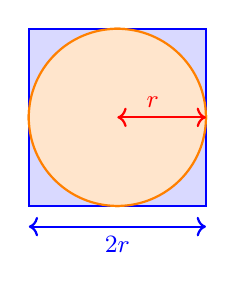
\begin{tikzpicture}[scale=0.75]
  \draw[thick, blue] (0,0) rectangle (3,3);
  \draw[thick, orange] (1.5,1.5) circle (1.5cm);
  \fill (1.5,1.5) circle (0.04);

  % Shade corners to show wasted space
  \begin{scope}
    \clip (0,0) rectangle (3,3);
    \fill[blue!15] (0,0) rectangle (3,3);
    \fill[orange!20] (1.5,1.5) circle (1.5cm);
  \end{scope}
  \draw[thick, blue] (0,0) rectangle (3,3);
  \draw[thick, orange] (1.5,1.5) circle (1.5cm);

  \draw[red, thick, <->] (1.5,1.5) -- ++(0:1.5);
  \node[red] at (2.1,1.75) {\small $r$};
  \draw[blue, thick, <->] (0,-0.35) -- (3,-0.35);
  \node[blue] at (1.5,-0.65) {\small $2r$};

\end{tikzpicture}
\end{center}

\column{0.65\textwidth}
\small
\begin{enumerate}
  \begin{multicols}{2}
    \item $5 \times 5 = \ashowq{25}$
    \item $8^2 = \ashowq{64}$
  \end{multicols}
  \begin{multicols}{2}
    \item $2.5^2 = \ashowq{6.25}$
    \item $3.14 \times 9 = \ablank{28.26}$
  \end{multicols}
  \item Area of a $7$ cm $\times$ $4$ cm rectangle $= \ashowq{28\,\text{cm}^2}$
  \item What fraction of $360^\circ$ is $90^\circ$? \ashow{$\frac{1}{4}$}
\end{enumerate}

\begin{enumerate}
  \setcounter{enumi}{6}
  \item Write an expression for the area of the circle in the picture \ashow{$\pi r^2$}
  \item Write an expression for the area of the shaded blue region in the picture \ashow{$4r^2-\pi r^2$}
  \item If the square has a perimeter of 48cm, what is the area of the shaded blue region? \ashow{$30.96\,\text{cm}^2$}
\end{enumerate}

\end{columns}
\end{frame}

\begin{frame}{Worked Solution: Starter 3, Question 1}
\hypertarget{work-st3}{}
\textbf{Question:} \(5 \times 5 = \ashowq{25}\)

\textbf{Worked Solution:} \ashow{\(5 \times 5 = 25\).}
\end{frame}

\begin{frame}{Worked Solution: Starter 3, Question 2}
\textbf{Question:} \(8^2 = \ashowq{64}\)

\textbf{Worked Solution:} \ashow{\(8^2 = 8 \times 8 = 64\).}
\end{frame}

\begin{frame}{Worked Solution: Starter 3, Question 3}
\textbf{Question:} \(2.5^2 = \ashowq{6.25}\)

\textbf{Worked Solution:} \ashow{\(2.5 \times 2.5 = 6.25\).}
\end{frame}

\begin{frame}{Worked Solution: Starter 3, Question 4}
\textbf{Question:} \(3.14 \times 9 = \ablank{28.26}\)

\textbf{Worked Solution:} \ashow{\(3.14 \times 9 = 3.14 \times (10-1) = 31.4 - 3.14 = 28.26\).}
\end{frame}

\begin{frame}{Worked Solution: Starter 3, Question 5}
\textbf{Question:} Area of a \(7\) cm \(\times\) \(4\) cm rectangle \(= \ashowq{28\,\text{cm}^2}\)

\textbf{Worked Solution:} \ashow{\(7 \times 4 = 28\), so the area is \(28\,\text{cm}^2\).}
\end{frame}

\begin{frame}{Worked Solution: Starter 3, Question 6}
\textbf{Question:} What fraction of \(360^\circ\) is \(90^\circ\)?

\textbf{Worked Solution:} \ashow{\(\frac{90}{360} = \frac{1}{4}\).}
\end{frame}

\begin{frame}{Worked Solution: Starter 3, Question 7}
\textbf{Question:} Write an expression for the area of the circle in the picture, which has radius \(r\).

\textbf{Worked Solution:} \ashow{\(A = \pi r^2\).}
\end{frame}

\begin{frame}{Worked Solution: Starter 3, Question 8}
\textbf{Question:} Write an expression for the area of the shaded blue region in the picture, where the square has side \(2r\) and the circle has radius \(r\).

\textbf{Worked Solution:} \ashow{Square area \(= (2r)^2 = 4r^2\). Shaded area \(= 4r^2 - \pi r^2\).}
\end{frame}

\begin{frame}{Worked Solution: Starter 3, Question 9}
\textbf{Question:} If the square has a perimeter of \(48\) cm, what is the area of the shaded blue region?

\textbf{Worked Solution:} \ashow{Side \(= 48 \div 4 = 12\) cm, so \(2r = 12\) and \(r = 6\) cm. Square area \(= 12^2 = 144\) cm\(^2\). Circle area \(= \pi \times 6^2 = 3.14 \times 36 = 113.04\) cm\(^2\). Shaded area \(= 144 - 113.04 = 30.96\) cm\(^2\).}
\end{frame}

%------------------------------------------------
% STARTER 4
%------------------------------------------------
\begin{frame}{Starter 4}
\hypertarget{q-st4}{}

\vspace{-1em}

\begin{columns}

\column{0.35\textwidth}
\begin{center}
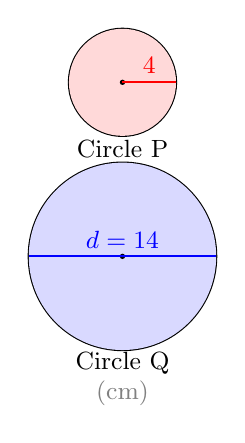
\begin{tikzpicture}[scale=0.85]

  % Two circles for comparison
  \draw[thick] (0, 2.2) circle (0.8cm);
  \fill[red!15] (0,2.2) circle (0.8cm);
  \fill (0,2.2) circle (0.04);
  \draw[red, thick] (0,2.2) -- ++(0:0.8);
  \node[red] at (0.4, 2.45) {\small $4$};
  \node at (0, 1.2) {\small Circle P};

  \draw[thick] (0,-0.4) circle (1.4cm);
  \fill[blue!15] (0,-0.4) circle (1.4cm);
  \fill (0,-0.4) circle (0.04);
  \draw[blue, thick] (-1.4,-0.4) -- (1.4,-0.4);
  \node[blue] at (0,-0.15) {\small $d=14$};
  \node at (0,-2.0) {\small Circle Q};

  \node[gray] at (0,-2.45) {\small (cm)};

\end{tikzpicture}
\end{center}

\column{0.65\textwidth}
\small
\begin{enumerate}
  \begin{multicols}{2}
    \item $9^2 = \ashowq{81}$
    \item $3.5^2 = \ashowq{12.25}$
  \end{multicols}
  \begin{multicols}{2}
    \item $3.14 \times 16$ \ashow{$=50.24$}
    \item $3.14 \times 49$ \ashow{$=153.86$}
  \end{multicols}
  \item Halve $14$ cm. \quad Then square your answer. \ashow{$7$ cm, so $49\,\text{cm}^2$}
  \item A square has area $64$ cm$^2$. What is its side length \ashowq{$8$ cm}
\end{enumerate}

\begin{enumerate}
  \setcounter{enumi}{6}
  \item \textbf{Spot the mistake:} \textit{``Circle Q has diameter $14$ cm, so its area is $\pi \times 14^2 \approx 615$ cm$^2$.''} What error was made? Write the correct solution. \ashow{Used diameter not radius: $\pi \times 7^2 \approx 153.86\,\text{cm}^2$.}
  \item \textbf{Circle P}, radius $4$ cm. Find: (a) the area \ablank{$50.24\,\text{cm}^2$} \quad (b) the circumference \ablank{25.12\,\text{cm}}.
  \item \textbf{Circle Q}, diameter $14$ cm. Find: (a) the area \ablank{$153.86\,\text{cm}^2$} \quad (b) the circumference \ablank{43.96\,\text{cm}}.
  \item Which has the greater area, P or Q? By approximately how many cm$^2$? \ashow{Q, by approximately $103.62\,\text{cm}^2$.}
\end{enumerate}

\end{columns}
\end{frame}

\begin{frame}{Worked Solution: Starter 4, Question 1}
\hypertarget{work-st4}{}
\textbf{Question:} \(9^2 = \ashowq{81}\)

\textbf{Worked Solution:} \ashow{\(9^2 = 9 \times 9 = 81\).}
\end{frame}

\begin{frame}{Worked Solution: Starter 4, Question 2}
\textbf{Question:} \(3.5^2 = \ashowq{12.25}\)

\textbf{Worked Solution:} \ashow{\(3.5 \times 3.5 = \frac{7}{2} \times \frac{7}{2} = \frac{49}{4} = 12.25\).}
\end{frame}

\begin{frame}{Worked Solution: Starter 4, Question 3}
\textbf{Question:} \(3.14 \times 16 = ?\)

\textbf{Worked Solution:} \ashow{\(3.14 \times 16 = 3.14 \times (10 + 6) = 31.4 + 18.84 = 50.24\).}
\end{frame}

\begin{frame}{Worked Solution: Starter 4, Question 4}
\textbf{Question:} \(3.14 \times 49 = ?\)

\textbf{Worked Solution:} \ashow{\(49 = 50 - 1\), so \(3.14 \times 49 = 3.14 \times 50 - 3.14 = 157 - 3.14 = 153.86\).}
\end{frame}

\begin{frame}{Worked Solution: Starter 4, Question 5}
\textbf{Question:} Halve \(14\) cm, then square your answer.

\textbf{Worked Solution:} \ashow{Halving gives \(14 \div 2 = 7\) cm. Squaring gives \(7^2 = 49\), so the answer is \(49\,\text{cm}^2\).}
\end{frame}

\begin{frame}{Worked Solution: Starter 4, Question 6}
\textbf{Question:} A square has area \(64\) cm\(^2\). What is its side length? \ashowq{\(8\) cm}

\textbf{Worked Solution:} \ashow{Since \(8^2 = 64\), the side length is \(\sqrt{64} = 8\) cm.}
\end{frame}

\begin{frame}{Worked Solution: Starter 4, Question 7}
\textbf{Question:} Spot the mistake: \textit{``Circle Q has diameter \(14\) cm, so its area is \(\pi \times 14^2 \approx 615\) cm\(^2\).''} What error was made? Write the correct solution.

\textbf{Worked Solution:} \ashow{The diameter was used instead of the radius. The radius is \(14 \div 2 = 7\) cm, so the correct area is \(\pi \times 7^2 = 3.14 \times 49 \approx 153.86\) cm\(^2\).}
\end{frame}

\begin{frame}{Worked Solution: Starter 4, Question 8}
\textbf{Question:} Circle P has radius \(4\) cm. Find: (a) the area \ablank{\(50.24\,\text{cm}^2\)} and (b) the circumference \ablank{\(25.12\,\text{cm}\)}.

\textbf{Worked Solution:} \ashow{\(A = \pi r^2 = 3.14 \times 4^2 = 3.14 \times 16 = 50.24\) cm\(^2\). \(C = 2\pi r = 2 \times 3.14 \times 4 = 25.12\) cm.}
\end{frame}

\begin{frame}{Worked Solution: Starter 4, Question 9}
\textbf{Question:} Circle Q has diameter \(14\) cm. Find: (a) the area \ablank{\(153.86\,\text{cm}^2\)} and (b) the circumference \ablank{\(43.96\,\text{cm}\)}.

\textbf{Worked Solution:} \ashow{Radius \(= 14 \div 2 = 7\) cm. \(A = \pi r^2 = 3.14 \times 7^2 = 3.14 \times 49 = 153.86\) cm\(^2\). \(C = \pi d = 3.14 \times 14 = 43.96\) cm.}
\end{frame}

\begin{frame}{Worked Solution: Starter 4, Question 10}
\textbf{Question:} Which has the greater area, P or Q? By approximately how many cm\(^2\)?

\textbf{Worked Solution:} \ashow{Area P is \(50.24\) cm\(^2\), and area Q is \(153.86\) cm\(^2\). Therefore Q is greater by \(153.86 - 50.24 = 103.62\) cm\(^2\).}
\end{frame}

\end{document}